\documentclass[twoside,single]{lion-msc}

\title{Summer Research Internship 2017}
\author{Mudit Garg}

\affiliation{Indian Institute of Technology Delhi}   % this is the default value
%\affiliation{Instituut-Lorentz, Leiden University}                     % for theoretical physics
\usepackage{float}
%\affiliation{Huygens-Kamerlingh Onnes Laboratorium, Universiteit Leiden}   % experimental physics in Dutch
%\affiliation{Instituut-Lorentz, Universiteit Leiden}                       % theoretical physics in Dutch
\id{Senior Undergraduate}
\address{New Delhi, India, 110016}               % default address - uncomment if need be
\usepackage{amssymb} 
\usepackage[export]{adjustbox}
% \newdate{date}{\day}{\month}{\year}           % definition of time and date using datetime package
%\newdate{date}{27}{08}{2010}
%\date{\displaydate{date}}
\usepackage{enumerate}
\studentid{May-July 2017}                           % check you student ID, LaTeX does not do this
\abstract{I would like to express my deep gratitude toward \textbf{Prof. Michel Orrit} for giving me this wonderful opportunity to spend my Summer at Single Molecule Group and for his constant guidance.I would like to thank \textbf{Biswajit Pradhan} for his daily supervision and constructive discussions .\\~\\
This research internship was made possible by financial support from the \textbf{Leiden University} and I am thankful for that.I am certainly grateful to \textbf{Prof. Jan Aarts} for coordinating my summer internship and taking care of all logistics.
\\~\\Special thanks to \textbf{MoNOS} group for accepting me in their family and helping me into smooth transition in leiden.I've gained so much experience and knowledge here that can't be expressed in words. \\~\\
Also I  would like to express my gratitude toward  \textbf{Prof. R.K. Soni}, the internal supervisor of this internship with his ever-helping nature and support.   }     % limit your self to 1/2 page or 500 words
\supervisor{Prof. Dr. Michel Orrit}                         % Note that this should be a LION staff member!
\dsupervisor{Biswajit Pradhan}                      % This could be a LION staff member or your external supervisor

\degree{Research Internship}                     % The default option is "Bachelor of Science", change if needed


\major{Single-Molecule Group,LION}                  % The default option is "Physics", change if needed
%\major{Physics and Mathematics}

% optional cover picture - should be jpg or pdf

\coverpicture{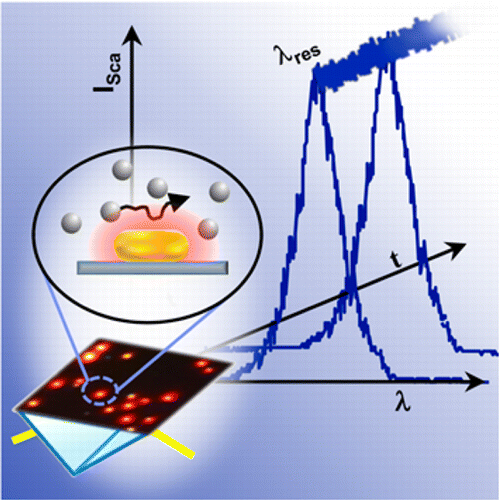
\includegraphics[width=8cm]{1.png}} 


% Use this to make hyperlinks visible in the document.
% \hypersetup{colorlinks=true}

% ---------------------------------------------------------------- My defintions!
% \renewcommand{\vec}[1] {\ensuremath{ \overrightarrow{ #1 } }}
\renewcommand{\vec}[1] {\ensuremath{ \mathbf{ #1 } }}
% \bra \ket \braket and \proj
\newcommand{\bra}[1]{\ensuremath{\langle #1 \vert}}
\newcommand{\ket}[1]{\ensuremath{\vert #1 \rangle}}
\newcommand{\braket}[2]{\ensuremath{\langle #1 \vert #2 \rangle}}
\newcommand{\proj}[1]{\ensuremath{\vert #1 \rangle \langle #1 \vert}}

\newcommand{\kpar}{\ensuremath{k_\parallel}}
% ----------------------------------------------------------------

% \usepackage{tocloft}
% \renewcommand{\cftchapdotsep}{\cftdotsep}

\begin{document}

% roman numbering in the table of contents section
\pagenumbering{roman}


\maketitle

% Table of contents :  it is a good idea to include this into your thesis
\tableofcontents
\cleardoublepage

% The following list of figures and list of tables are optional. Remove the comments if needed
%\listoffigures
%\newpage

%\listoftables
%\newpage

% in the main part of the document use standard arabic numbers. Page counter resets to 1.
\pagenumbering{arabic}

\chapter{Introduction}

In this Internship I've used Fluorescence Correlation Spectroscopy to observe the single Gold nanorods(AuNR) as they interact with their nearby particles like proteins,silica nanoparticles.\cite{AuNR1} .I first learned how to operate the system and how to make samples for the system.Then I learned how to take spectrum using luminescence with the help of 532nm green laser.By analyzing the spectrum I used appropriate AuNR to take their spectrum image with 660nm cobalt laser. Then I introduces BSA of different concentration. in environment of AuNR .I took time traces using two APDs and try to observe some bursts in that. There were some problems which I will discuss in Result section.

\chapter{Theory}

\section{Fluorescence}
Fluorescence is the property of substance where it absorbs light at certain  wavelength and emit light at relatively longer wavelength,Therefore have lower energy than the absorbed one.Molecule is termed as fluorophores or fluorescent dyes.It happens in three stages : First Excitation then Excited state Lifetime and finally Fluorescence Emission.This is displayed using Jablonski diagram.More details are in this reference \cite{AuNR2} \\
\\
\begin{center}
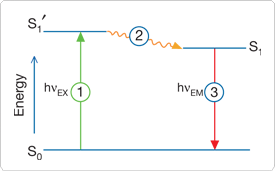
\includegraphics[scale=1]{2.png}\\
Jablonski diagram:Three stages of Fluorescence \cite{AuNR2} 
\end{center}

\section{Fluorescence Correlation Spectroscopy}
Fluorescence Correlation Spectroscopy(FCS) is a technique which can be used to monitor single molecule using specific optical setup with an inverted confocal microscope.In this setup we send laser beam to this microscope's objective via Beam splitter,which focus on the sample.Then we gather the fluorescence light form this and send it to pin hole and via emissions filters and beam splitter which use few nanomolars of fluorescence in order to detect single molecule.Then we use two APD detectors which are getting light from 50/50 beam splitter then take their cross correlation.Formula for normalized autocorrelation of intensity i.e. I(t) is :
$$
G(\tau) = \frac{\langle{I(t)}\cdot{I(t+\tau)}\rangle}{\langle{I(t)}\rangle^2} 
$$
and if we define $\delta{I(t)} = I(t) - \langle{I(t)}\rangle$ then $G(\tau)$ can be written as :
$$
G(\tau) = \frac{\langle\delta{I(t)}\cdot\delta{I(t+\tau)}\rangle}{\langle{I(t)}\rangle^2} +1
$$
It is given in more details in reference \cite{AuNR3}


\section{Scattering Correlation Spectroscopy}
In this technique\cite{AuNR1} we monitor an immobilized single AuNR using scattering from the white light using the TIE configuration.We use flow cell to control the environment of the AuNR. Then we introduce diffusers such as small gold.We measure the shift in spectra of the AuNR as diffusers enter and leaves in its vicinity.Then we take autocorrelation of $\lambda(t)$ in to find out diffusion coefficient D.Then using stokes einstein relation $ D = \frac{k_B{T}}{6\pi\eta{r}}$ we can find viscosity and diffuser conc. of other diffusers if we know it for one using their respective D.
$$
G(\tau) -1= \frac{\langle\delta\lambda(t) \cdot\delta\lambda(t+\tau) \rangle}{\langle{\lambda(t)}\rangle^2}
$$
\begin{figure}[H]
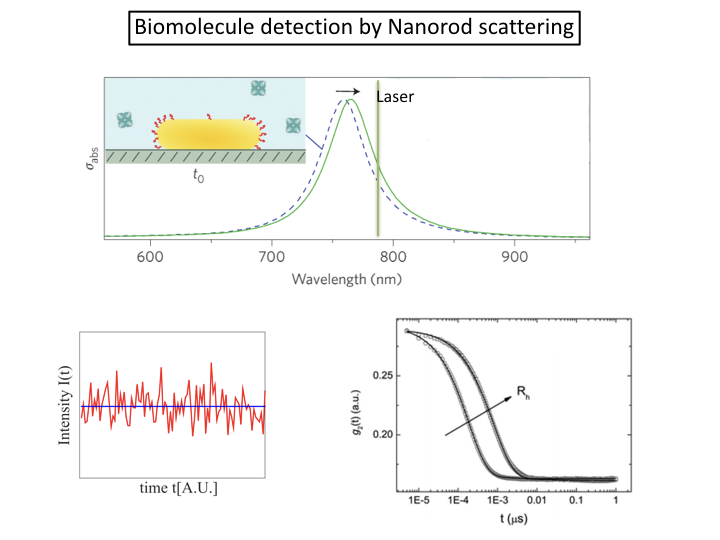
\includegraphics[width=1\textwidth,left]{13}
Shift in spectrum \& correlation due to protein in the vicinity of AuNR\cite{AuNR4}
\end{figure}

\begin{figure}[H]
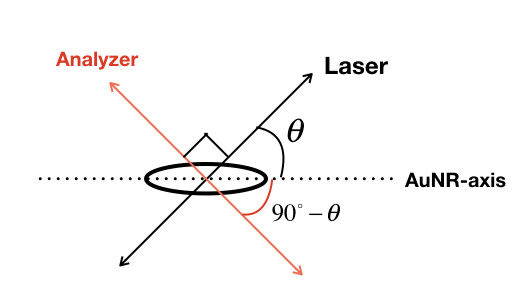
\includegraphics[width=1\textwidth,left]{9}
\end{figure}

Laser is at an angle $\theta$ with axis of AuNR and perpendicular to analyzer which is extinguishing the reflection part (
$ I_{reflection} = = I_{L}\cdot\cos90^{\circ} = 0$) .so only scattering along the axis survive and result in final intensity.
$$
I_{total} = Reflection+AuNR-scat = 0 +   I_{scatAuNR}\cdot\cos(90^{\circ}-\theta)
$$
$$
I_{total} = I_{scatAuNR}\cdot\sin(\theta)
$$
\section{Procedure}
This is my full procedure in the internship:
\begin{enumerate}[A.]
\item \textbf{Sample Preparation}
 \begin{enumerate}[I]
   \item I first prepared sample using stock AuNR solution which were coated with CTAB to avoid aggregates
   \item I only chose those solution which have surface plasmon resonance around 650 so that they right swing at 660nm.
   \item then remove CTAB using centrifugation.This is necessary so that AuNR could stuck glass slides.
   \item then I sonicated the sample to avoid aggregates.
   \end{enumerate}
   \item \textbf{Putting AuNRs on glass slide}
   \begin{enumerate}[I]
   \item After that I used two different things to put AuNR sample
   \begin{enumerate}[i]
   \item Flow cell with rectangular slide
   \item Circular holder with circular slides
   \end{enumerate}
   \item Also used two different procedure for introducing AuNR to glass slides
   \begin{enumerate}[i]
   \item Spin coating method 
   \item Flowing AuNR solution into flow cell
   \end{enumerate}
   \end{enumerate}
   \item \textbf{Experimenting}
     \begin{enumerate}[I]
   \item So I used this setup for experimenting
   \begin{figure}[H]
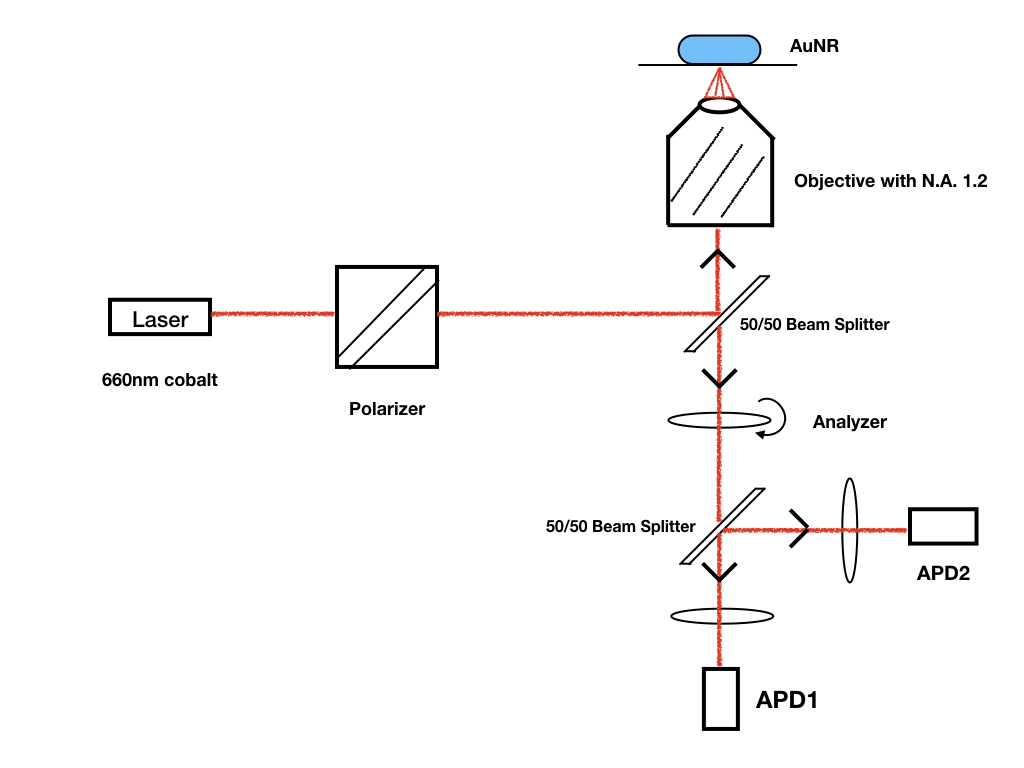
\includegraphics[width=1.1\textwidth,left]{10}
\begin{flushleft}
In this Experimental setup laser is going through polarizer then using 50/50 beam splitter going to AuNR though microscope and coming back through analyzer which is then again splitting by 50/50 beam splitter to APDs. 
\end{flushleft}
\end{figure}
   \item I took scattering image using 660nm red laser at focus for finding out positions of AuNR.
   \item Then I took spectrum using 532nm green laser for those AuNR which were excited by 660nm.
   \item After doing this process I chose those AuNRs which had SPR either right swing or left wing at 660nm.
   \item then I passivated the AuNRs with either Thioglycolic acid or Cysteamine to avoid physical contact between protein and AuNR.
   \item Then after leaving it for overnight I introduces different conc. of BSA protein.
   \item Took their time traces using two APDs.
   \end{enumerate}
   \item \textbf{Analysis}
   \begin{enumerate}[I]
   \item I found out their cross correlations using time traces in order to find diffusion time.
   \item and finally using Stokes Einstein relation to find out size of protein.
    \end{enumerate}
   \end{enumerate}
\chapter{Results and Discussion}

As I laid out in my procedure in previous chapters,I was not able to achieve them perfectly this was due to these things:
\begin{enumerate}
\item Time constraint of my internship
\item initially laser wasn't stable
\item Not able to prevent attaching of BSA to AuNR
\end{enumerate}
Due to this time constraint I spent my initial time learning the technique and how to make samples.After that we found out that our 670nm laser is not stable,so we ordered a new one 660nm cobalt laser but even after accelerating the procedure it took 3 weeks to arrive.even after finally setting up the laser which was stable.we weren't able to avoid attaching of BSA even after the passivation.So I would like to share my two days of result in which laser was stable.So in first case I passivated with 20$\mu$M Cysteamine and in second case with 100 $\mu$M Thioglycolic acid.

\section{Passivation with 20$\mu$M Cysteamine}
\begin{center}
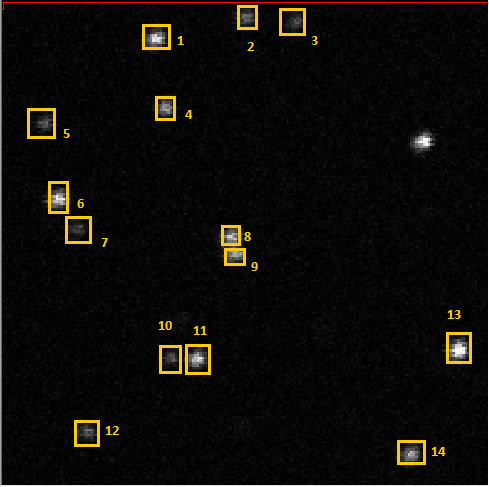
\includegraphics[scale=.75]{3.png}\\
Numbering according to order of taking spectrum
\end{center}
Out of these fifteen only ten i.e. 2,3,5,6,8,10,12,13,14,15 had right spectrum.
then I introduced 100nM BSA.Then took 300 second time traces.After doing that I again took the spectra and found out that there was a shift of 2-3nm in SPR and decrease of around 1nm in FWHM.
\begin{center}
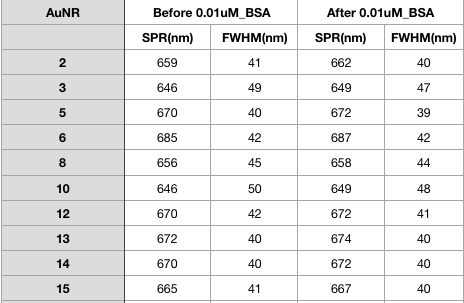
\includegraphics[scale=.6]{4.png}\\
Change in Spectrum before and after introduction of BSA
\end{center}
I would particularly discuss one of the AuNR which was showing some correlation i.e. AuNR6
\begin{figure}[h]
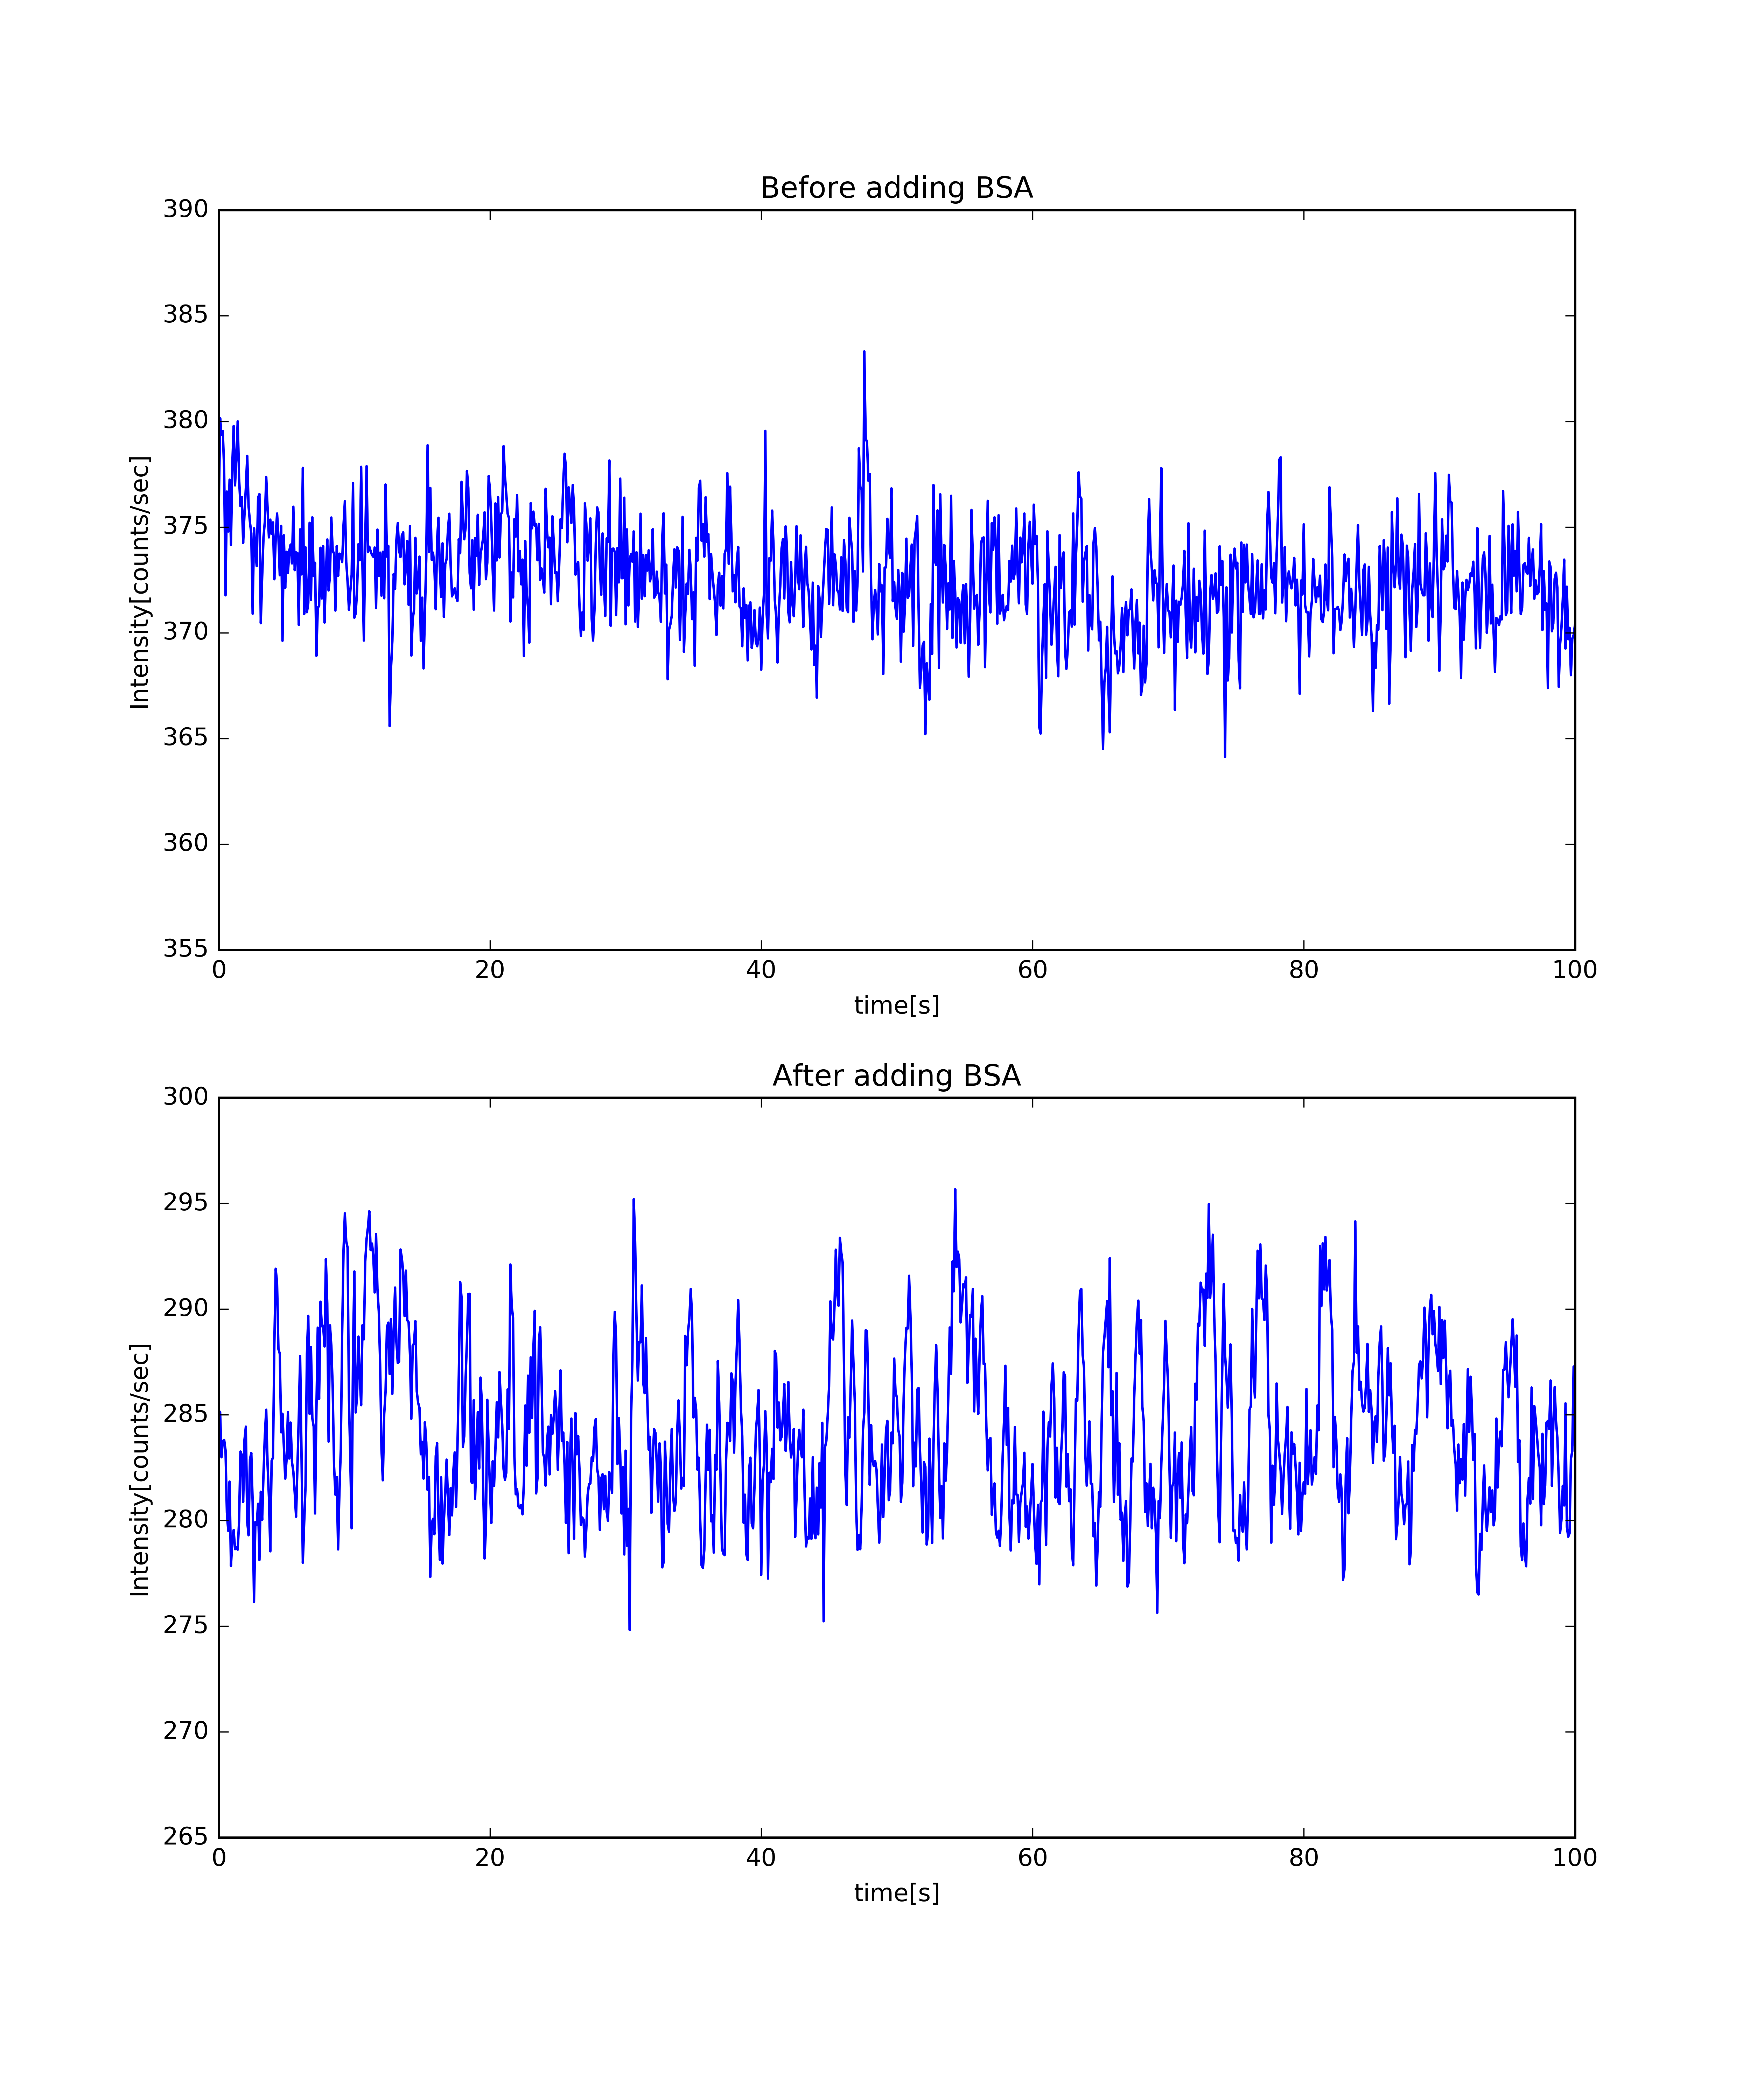
\includegraphics[width=.8\textwidth,center]{11}
\begin{center}
Time Trace of 6 before and after BSA.As we can see from time traces that due to BSA there are fluctuations in this
\end{center}
\end{figure}
\begin{figure}[h]
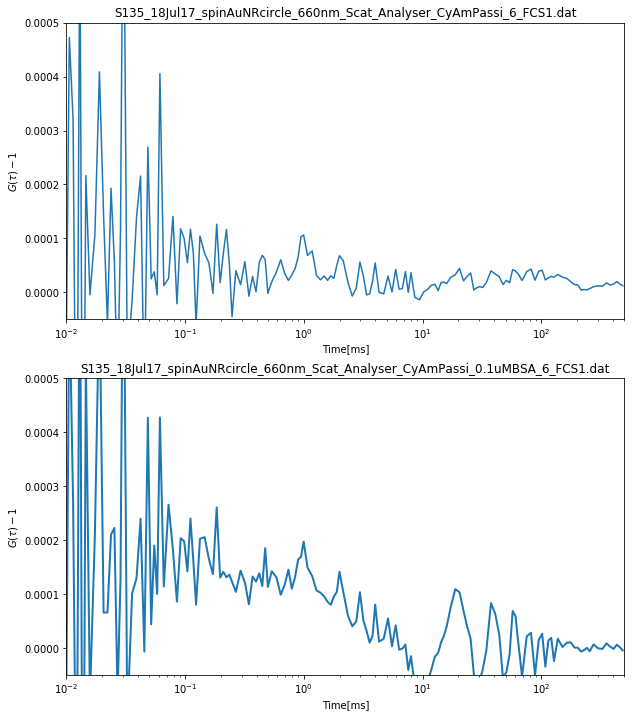
\includegraphics[width=.8\textwidth,center]{12}
\begin{center}
FCS correlations of AuNR6 before and after BSA.There is some correlation due to the some sticking of BSA
\end{center}
\end{figure}

\begin{figure}[h]
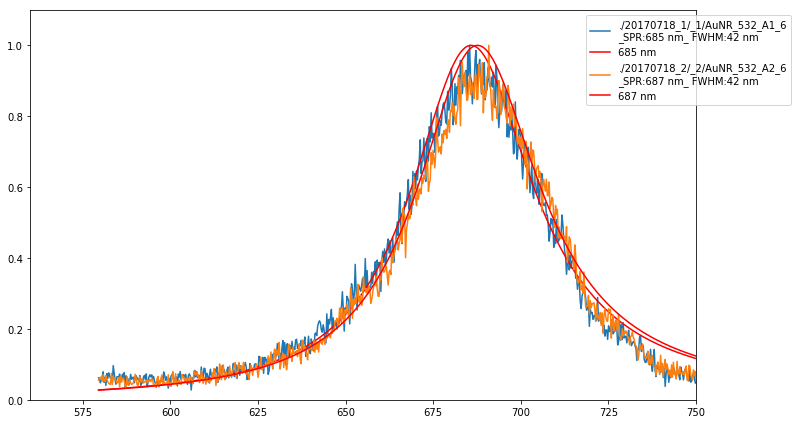
\includegraphics[width=.8\textwidth,center]{7}
\begin{center}
Spectrum shift in AuNR6 before and after BSA.
\end{center}
\end{figure}
\section{Passivation with 100$\mu$M Cysteamine}
\begin{center}
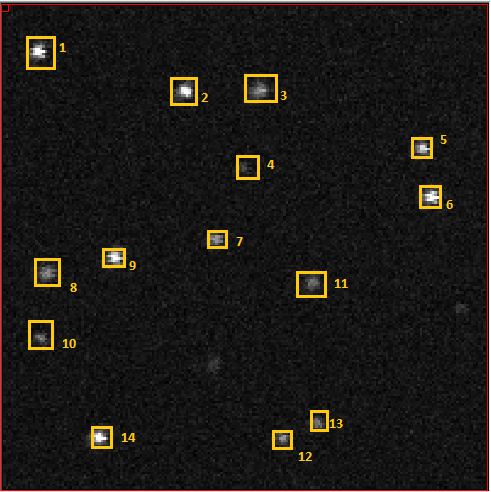
\includegraphics[scale=.75]{6.png}\\
Numbering according to order of taking spectrum
\end{center}
Out of these fourteen only nine i.e. 1,3,4,6,7,10,11,12,13 had right spectrum.
then I introduced 1nM BSA.Then took 600 second time traces.After doing that I again took the spectra and found out that there was a shift of 2-3nm in SPR and but his time increase of around 1nm in FWHM.
\begin{center}
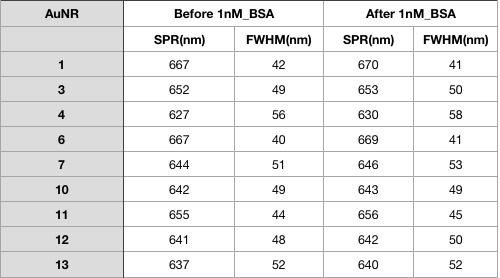
\includegraphics[scale=.6]{5.png}\\
Change in Spectrum before and after introduction of BSA
\end{center}

\section{Conclusion}
First conclusion is that we're experimentally able to detect protein sticking with our theory.Second conclusion is that due to only maximum 3-4 \% increase in time trace after introduction of BSA ,FCS correlation is too noisy which hinders our ability to analyze.
 
\section{Outlook}
We can use good detectors which have low noises such as photodiode to get better idea from correlations.Also we can passivate AuNR better to avoid sticking with protein.
\bibliographystyle{lion-msc}
\bibliography{Thesis}

\end{document}

